\documentclass[../../main.tex]{subfiles}
\graphicspath{{../../image/}{../../figure/}}
\begin{document}

\section{弱解的崩坏}\label{section:ch09-弱解的崩坏}

如前节所见,波碰撞可能诱发波放大。下例表明,由此产生共振波型,在有限时间内驱动弱解的振荡和/或全变差趋于无穷。

考虑方程组
\begin{align}
\begin{cases}
\partial_{t}u+\partial_{x}(uv+w)=0,\\
\partial_{t}v+\partial_{x}\big(\frac{1}{16}v^{2}\big)=0,\\
\partial_{t}w+\partial_{x}(u-uv^{2}-vw)=0.
\end{cases}
\label{align:ch09-9-10-1}
\end{align}
特征速度为 $\lambda_{1}=-1$, $\lambda_{2}=\frac{1}{8}v$, $\lambda_{3}=1$,故当 $-8<v<8$ 时严格双曲成立。第一与第三特征族线性退化,而第二特征族真正非线性。显然该方程组部分解耦:类 Burgers 的第二方程独自确定 $v$。

速度为 $s$、连接左状态 $(u_{-},v_{-},w_{-})$ 与右状态 $(u_{+},v_{+},w_{+})$ 的激波,其 Rankine-Hugoniot 跳跃条件在此为
\begin{align}
\begin{cases}
u_{+}v_{+}-u_{-}v_{-}+w_{+}-w_{-}=s(u_{+}-u_{-}),\\
\frac{1}{16}v_{+}^{2}-\frac{1}{16}v_{-}^{2}=s(v_{+}-v_{-}),\\
u_{+}-u_{-}-u_{+}v_{+}^{2}+u_{-}v_{-}^{2}-v_{+}w_{+}+v_{-}w_{-}=s(w_{+}-w_{-}).
\end{cases}
\label{align:ch09-9-10-2}
\end{align}
易见 1-激波即 1-接触间断, $s=-1$, $v_{-}=v_{+}$,且
\begin{align}
w_{+}-w_{-}=-(v_{\pm}+1)(u_{+}-u_{-}).
\label{align:ch09-9-10-3aa}
\end{align}
类似地,3-激波即 3-接触间断, $s=1$, $v_{-}=v_{+}$,且
\begin{align}
w_{+}-w_{-}=-(v_{\pm}-1)(u_{+}-u_{-}).
\label{align:ch09-9-10-3ab}
\end{align}
最后,对 2-激波, $s=\frac{1}{16}(v_{-}+v_{+})$,且 $v_{+}<v_{-}$,以满足 Lax $E$ 条件。

连接常状态的任意两激波碰撞产生一个跳跃间断,可通过求解简单 Riemann 问题化解。特别地,当 1-激波或 3-激波与 2-激波碰撞时,2-激波不受扰动,因为\eqref{align:ch09-9-10-1}$_{2}$ 与方程组另两方程解耦。然而这种碰撞产生出射的 1-激波与 2-激波,可解释为入射 1-或 2-激波的"透射"部分与"反射"部分。

现构造\eqref{align:ch09-9-10-1}的一个分片常数、容许解,其波型如图\ref{figure:ch09-弱解共振波型}所示:从点 $(-1,0)$ 与 $(1,0)$ 各发出一个 2-激波,速度分别为 $\frac{1}{4}$ 与 $-\frac{1}{4}$。在左 2-激波左侧, $v=4$;在右 2-激波右侧, $v=-4$;两 2-激波之间, $v=0$。一个 1-激波从原点 $(0,0)$ 发出,与左 2-激波碰撞时部分透射为 1-激波、部分反射为 3-激波。此 3-激波击上右 2-激波时,又部分透射为 3-激波、部分反射为 1-激波,过程无限重复。

\begin{figure}[ht]
\centering
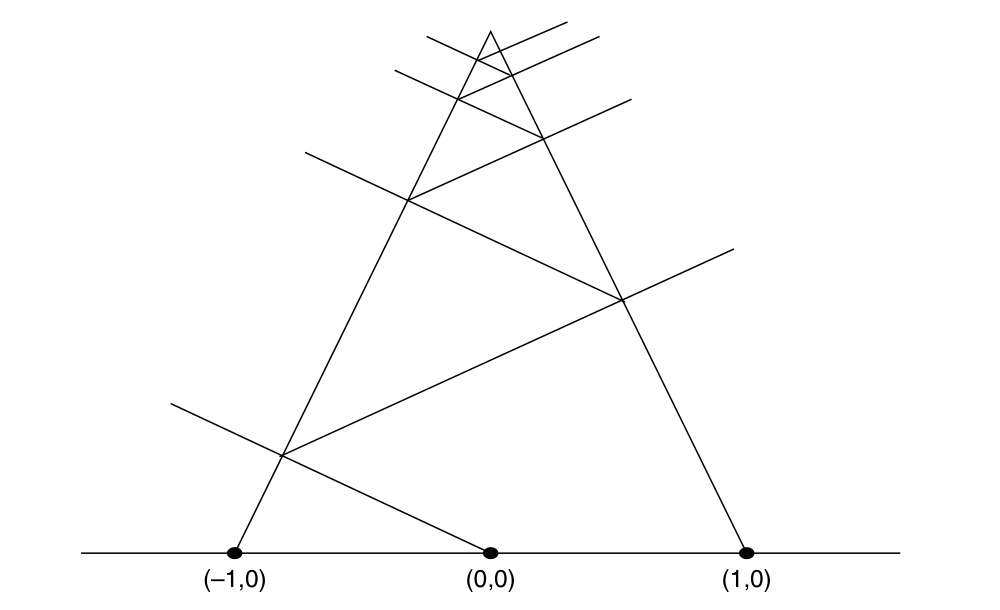
\includegraphics[width=0.62\textwidth]{ch09-fig10-01.png}
\caption{弱解共振波型:两 2-激波与反复透射-反射的 1-/3-激波。}
\label{figure:ch09-弱解共振波型}
\end{figure}

通过核验 Rankine-Hugoniot 条件\eqref{align:ch09-9-10-2},易验证初值
\begin{align}
(u(x,0),v(x,0),w(x,0))=
\begin{cases}
(-65,+4,+225),&-\infty<x<-1,\\
(+15,0,-15),&-1<x<0,\\
(-15,0,+15),&0<x<1,\\
(-63,-4,-225),&1<x<\infty
\end{cases}
\label{align:ch09-9-10-4}
\end{align}
产生具上述结构的解。

目的是证明每次反射以常数因子增强激波强度。由于两 2-激波间距随时间减小,碰撞越来越频繁,最终在 $t=4$ 处消失,于是结论是:解的振荡当 $t\uparrow4$ 时爆炸。方便起见,用 $u$ 跨越 1-与 3-激波的跳跃大小来度量其强度。

先考察图\ref{figure:ch09-1激波碰左2激波}所描绘的相互作用,其中一个 1-激波从右侧击上左 2-激波。

\begin{figure}[ht]
\centering
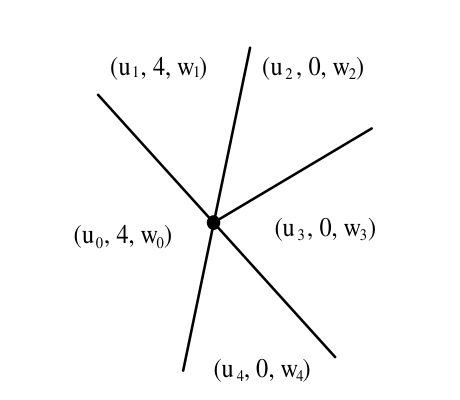
\includegraphics[width=0.42\textwidth]{ch09-fig10-02.png}
\caption{1-激波从右侧击上左 2-激波。}
\label{figure:ch09-1激波碰左2激波}
\end{figure}

需比较反射 3-激波的强度 $|u_{3}-u_{2}|$ 与入射 1-激波的强度 $|u_{3}-u_{4}|$。对相互作用中涉及的五个激波,按情况写出 Rankine-Hugoniot 条件\eqref{align:ch09-9-10-2}或\eqref{align:ch09-9-10-3aa}:
\begin{align}
\begin{cases}
w_{3}-w_{4}=-(u_{3}-u_{4}),\\
w_{1}-w_{0}=-5(u_{1}-u_{0}),\\
w_{3}-w_{2}=u_{3}-u_{2},\\
-4u_{0}+w_{4}-w_{0}=\frac{1}{4}(u_{4}-u_{0}),\\
u_{4}-u_{0}+16u_{0}+4w_{0}=\frac{1}{4}(w_{4}-w_{0}),\\
-4u_{1}+w_{2}-w_{1}=\frac{1}{4}(u_{2}-u_{1}),\\
u_{2}-u_{1}+16u_{1}+4w_{1}=\frac{1}{4}(w_{2}-w_{1}).
\end{cases}
\label{align:ch09-9-10-5}
\end{align}
经初等消元,得
\begin{align}
u_{3}-u_{2}=-\frac{10}{9}(u_{3}-u_{4}),
\label{align:ch09-9-10-6}
\end{align}
这表明 1-激波反射为 3-激波时,强度增大为 $10/9$ 倍。

接着考察图\ref{figure:ch09-3激波碰右2激波}所描绘的相互作用,其中一个 3-激波从左侧击上右 2-激波。再次写出完全类似于\eqref{align:ch09-9-10-5}的 Rankine-Hugoniot 条件,经直接消元,又得\eqref{align:ch09-9-10-6}。因而反射 1-激波的强度 $|u_{2}-u_{3}|$ 超过入射 3-激波的强度 $|u_{4}-u_{3}|$ 为 $10/9$ 倍。

\begin{figure}[ht]
\centering
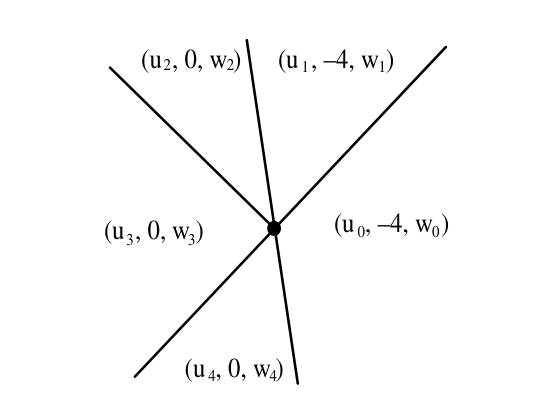
\includegraphics[width=0.42\textwidth]{ch09-fig10-03.png}
\caption{3-激波从左侧击上右 2-激波。}
\label{figure:ch09-3激波碰右2激波}
\end{figure}

于是我们已确认解的振荡当 $t\uparrow4$ 时爆炸。上述设定使计算格外简单,初看可能像一个孤立的奇例。然而,经过若干反射后即可看到,波共振在方程和/或初值的小扰动下持续存在,即这种类型的灾变可能是通有的。

也可能出现性质不同的灾变:即使振荡仍有界,全变差仍可能爆炸。这可在方程组
\begin{align}
\begin{cases}
\partial_{t}u+\partial_{x}(uv^{2}+w)=0,\\
\partial_{t}v+\partial_{x}\big(\frac{1}{16}v^{2}\big)=0,\\
\partial_{t}w+\partial_{x}(u-uv^{4}-v^{2}w)=0
\end{cases}
\label{align:ch09-9-10-7}
\end{align}
的框架中展示,它与\eqref{align:ch09-9-10-1}有相同特征速度,类似地允许具图\ref{figure:ch09-弱解共振波型}所示波型的分片常数解。可以调节两 2-激波的速度,使任两次相继反射后,1-与 3-激波恢复原来的左、右状态,即解在一个有限状态集合上取值。另一方面,当 $t$ 从下方趋近两 2-激波碰撞时刻 $t^{*}$ 时,穿越 $t$-时间线的固定强度激波数目无界增长,从而把全变差驱向无穷。细节见\cref{section:ch09-注记}所引文献。

鉴于上述,人们不应指望一般守恒律方程组在一般初值下 Cauchy 问题弱解的整体存在性。因而,理论的目标应是建立大范围内的存在性:要么对一般方程组在"小"初值下,要么对特殊方程组在一般初值下。希望这一特殊类别将包括连续物理中出现的、赋有特殊性质的方程组。

\end{document}
